\begin{problem}{Лесенки}{стандартный ввод}{стандартный вывод}{1 секунда}{256 мегабайт}

Лесенкой называется набор кубиков в один или несколько слоёв, в котором
каждый более верхний слой содержит кубиков меньше, чем нижний.

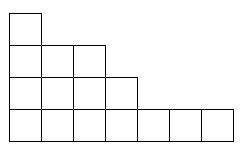
\includegraphics[scale=1,natwidth=243,natheight=152]{pic.jpg}

Подсчитать высоту лесенки из $N$ ступенек.

\InputFile
В первой строке записано число $N$ ($1 \le N \le 100$).

Во второй строке через пробел записаны $N$ положительных целых чисел, не превосходящих $10^9$~---~высоты ступенек в порядке невозрастания.

\OutputFile
Выведите одно целое число~---~высоту лесенки.

\Example

\begin{example}
\exmp{3
4 2 0
}{4
}%
\end{example}

\end{problem}

